\documentclass[12pt]{article}
\usepackage{amsmath,amssymb,amsthm}
\usepackage{fullpage}
\usepackage{graphicx}
\usepackage{hyperref}

\theoremstyle{definition}
\newtheorem{thm}{Theorem}[section]
\newtheorem{lem}[thm]{Lemma}
\newtheorem{defn}{Definition}[section]
\newtheorem{conj}{Conjecture}[section]
\newcommand{\floor}[1]{\left\lfloor #1 \right\rfloor}
\newcommand{\ceil}[1]{\left\lceil #1 \right\rceil}
\newcommand{\bigC}[0]{\mathcal{C}}
\begin{document}
\emergencystretch 3em
\title{
An attempt to connect Shannon's
circuit counting bound with clique detection}

\author{Josh Burdick}


\begin{abstract}
Shannon's function-counting argument
\cite{shannon_synthesis_1949} showed that some Boolean functions have
exponential circuit complexity, but doesn't provide a specific example
of such a hard-to-compute function. A simple modification of that argument
shows that detecting a randomly-chosen subset of the $k$-vertex cliques in an
$n$-vertex graph requires, on average, $\Omega(n^{k/2})$ NAND gates.
Unfortunately,
this doesn't directly bound the complexity of detecting {\em all} of the cliques; however, it seems like a
possibly related problem.
Here, we attempt to use random restrictions to approximately
connect the number of cliques detected, and the number of gates.
\end{abstract}

\maketitle

\newpage

\tableofcontents

This is an attempt to obtain a lower bound on detecting cliques
using NAND gates. Although it seems unlikely to work, hopefully
it will add to the long list of strange things which would happen
if P = NP (FIXME CITE).

\section{A counting bound}
\label{countingBound}

The first component we use is a slight modification
of Shannon's function-counting argument
\cite{shannon_synthesis_1949}.

\subsection{Background: lower bounds from function counting}

It has long been known that computing {\em some} function of a bit-string
requires exponentially large circuits \cite{shannon_synthesis_1949}.
Let $f: \{0,1\}^m \rightarrow \{0,1\}$ be a function from bitvectors to bits.
If there are $m$ inputs to a circuit,
then there are $2^{2^m}$ possible functions from the $m$-input bitstring to
a one-bit output. Each of these functions, being different, must have a
different circuit.

Given a count of functions, we can then see, for instance,
how many unbounded fan-in NAND gates are needed to compute
those functions (see Theorem \ref{boundFromCounting}
in Appendix \ref{gateMath}).

\subsection{Counting CLIQUE-like functions}

Suppose we are given an $n$-vertex graph.
Let $k$-CLIQUE($n$) be the boolean function which
detects $k$-cliques: it outputs 1 if any $k$-clique
is present, and 0 otherwise. This is a classic
NP-complete problem.

We now consider a ``buggy'' variant of the $k$-CLIQUE function,
which only detects a subset of cliques.
As a concrete example,
consider a set of ``buggy'' 6-clique finders. 
Maybe the circuit correctly
finds all the cliques. Or maybe it finds all of the cliques except $K_{1..6}$,
or it misses half the cliques, or finds none (and always outputs 0), or maybe
it only successfully finds $K_{1,3,4,5,7,8}$, et cetera.

We define a variant of $k$-CLIQUE which only
finds a subset of cliques.
Let $K$ denote the set of all possible
$k$-vertex cliques.

\begin{defn}
\label{BUGGYCLIQUE}
Let $A \subseteq K$.
Let $m = {n \choose 2}$ be the number of edges in the input graph.
$BUGGYCLIQUE(A): \{0,1\}^m \rightarrow \{0,1\}$ is the function which
is 1 iff any of the $K_k$s in $A$ is present 
That is, for each set $A$ of $K_k$s, $BUGGYCLIQUE(A)$
contains a function which is 1 if the input contains any $K_k \in A$,
and 0 otherwise. (Using this nomenclature,
$k$-CLIQUE(n) = $BUGGYCLIQUE(K)$).
\end{defn}

Of course, many of these functions are quite similar (e.g. all but one of them
output a 1 when you feed in all 1's). However, they're all slightly different.

\begin{thm}
\label{buggyDistinct}
There are  $2^{|K|}$ distinct $BUGGYCLIQUE$ functions.
\end{thm}
\begin{proof}

Let $A,B \subseteq K$, with $A \neq B$, and w.l.o.g.
let $x \in A-B$. Then $BUGGYCLIQUE(A)$ outputs 1 on the input
with just the edges in $x$ set to 1 (and 0 everywhere else),
while $BUGGYCLIQUE(B)$ outputs a 0.

There are $2^{|K|}$ many subsets of $K$,
and by the above, each corresponds to a diffferent function.
\end{proof}

For a given $A$, many of the functions in $BUGGYCLIQUE(A)$
are similar (for instance, most
of them output a 1 when all the edges are present);
but they are all distinct.
Although $2^{n \choose k}$ is a fairly large number,
it's still comfortably less than $2^{2^{n \choose 2}}$, the number of boolean
functions on the ${n \choose 2}$ input wires (one per edge).

\subsubsection{But {\em which} function requires many gates?}

Thus, there are $2^{n \choose k}$ different functions. 
How many NAND gates do these take?
(We consider NAND gate circuits (with any fan-in) which find $k$-cliques in $n$-vertex
graphs, as a circuit with $n \choose 2$ inputs)

Applying Theorem
\ref{boundFromCounting}, we know that at least one of the circuits requires
${\sqrt {2 {n \choose {k/2}} + b^2}} - b = \Omega(n^{k/2})$ 
NAND gates (where $b = {k \choose 2} - 0.5$).

Why doesn't this bound $k$-CLIQUE?
Because we don't know that the circuit which finds {\em all} of the
$K_k$s, is one of these larger circuits. As far as what I've
shown thus far goes, it could be harder to find some weird subset of the $K_k$s.

Indeed, as far as what we've formally shown goes, the problem which needs
the most NAND gates could be finding a single clique! That's easily ruled out
(because that only needs one NAND gate, plus the output gate).

\subsection{Which sets of cliques are hard to find?}
\label{sec:whichCliques}

The hardness of these functions depends
on how the cliques they find are laid out.

Cliques are arguably difficult to draw in a two-dimensional space.
As an approximate diagram reflecting what we know,
we sketch a Hasse diagram of possible subsets of cliques. Although
we only draw a few subsets of three-vertex cliques
on six vertices, hopefully this provides some
intuition.

\begin{figure}
\centering
\includegraphics[width=1\textwidth]{R/Hasse.pdf}
\caption{Hasse diagram of BUGGYCLIQUE functions.
(a-d) 
Detecting all the possible cliques in larger graphs will be
increasingly difficult (although {\em how much} harder isn't clear).
(e) 
Detecting this set of cliques is definitely harder than (b),
since we can convert from (e) to (b) by feeding in 0's to
some set of edges.
(f) Detecting a set of cliques which doesn't overlap much will be
harder than detecting the same number of cliques, when they overlap
maximally (as in (b)).}
\label{fig:Hasse}
\end{figure}


\begin{thm}
\label{edgeZonking}
Let $A \subsetneq B \subseteq K$, such that $A$ is what remains
of $B$ after removing all cliques overlapping some edge $e$.
Then $|\bigC(BUGGYCLIQUE(B))| > |\bigC(BUGGYCLIQUE(A))|$.
\end{thm}
\begin{proof}
Feed in a 0 to $e$ which is in $\bigC(B)$. The resulting
circuit computes $BUGGYCLIQUE(A)$, and so has size
at least $|\bigC(BUGGYCLIQUE(A))|$. But at least one
NAND gate has been removed by feeding in the 0.
\end{proof}

This shows that sometimes, finding a larger set of cliques is
harder. However, the above theorem doesn't help if the two
sets of cliques cover the same set of edges.

\begin{figure}
\label{overlappingTris}
\centering
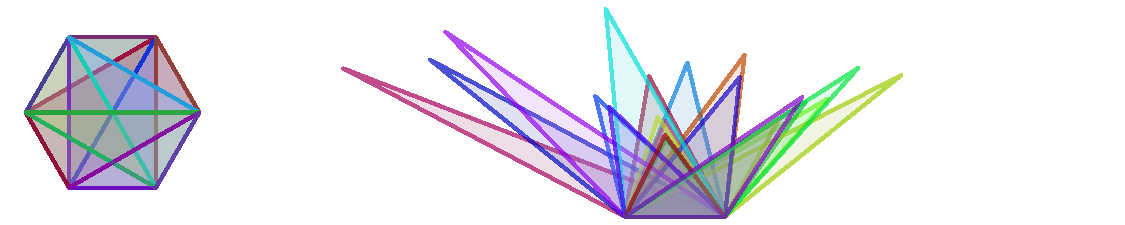
\includegraphics[width=1\textwidth]{R/tri1.pdf}
\caption{Sets of cliques which are highly overlapping (left),
or not overlapping much (right).}
\label{fig:overlappingTriangles}
\end{figure}

Triangles can be detected using matrix multiplication \cite{itai_finding_1977},
and there are fast algorithms known for matrix multiplication
\cite{strassen_gaussian_1969}
\cite{williams_multiplying_2012}, so the set of all possible
cliques on some set of vertices (Figure \ref{overlappingTris}, left)
 can be detected
using fewer than one NAND gate per triangle (for large enough input graphs).

On the other hand, if the triangles overlap less (as in
Figure \ref{overlappingTris}, right),
then to detect all of the triangles, we will definitely need at least one
gate per triangle. We can see this by feeding in a 0 to some input
unique to a triangle, applying \ref{edgeZonking}, and repeating.

\subsection{Defining levels of CLIQUE}

To me, it seems a reasonably intuitive guess that the hardness of
computing $BUGGYCLIQUE(A)$ should be somehow related to
$|A|$, which is simply the number of cliques it ``sees''.

\begin{defn}
\label{CLIQUE-level}
Assume $n, k$ are fixed. For any $l$ such that
$0 \le l \le |K|$, let $K_l$ be the set of all sets
with exactly $l$ cliques. 
\end{defn}

We abuse notation slightly, and write

\[
BUGGYCLIQUE(K_l) = \{ BUGGYCLIQUE(k) : k \in K_l \}
\]

What can we say about $E[|\bigC(BUGGYCLIQUE(K_l))|]$, for
some fixed $l$? Let $N = {n \choose k}$.
At the ``bottom'', there's only one $BUGGYCLIQUE(\emptyset)$
function, so the counting argument is useless.
In the ``middle'',
there are ${N \choose {N/2}}$ functions, and so the counting
argument gives a nontrivial lower bound for
$E[|\bigC(BUGGYCLIQUE(K_{N \choose {N/2}}))|]$ (although
without actually constructing even one difficult function).
At the ``top'', again, there's only one $BUGGYCLIQUE(K) = k-CLIQUE$
function, so the counting argument is, once again, useless.

It would be nice if we could show that, as $l$ increases,
$E[|\bigC(BUGGYCLIQUE(K_l))|]$ also increases.
If we could prove something in general, for all levels $l$, then at
the top of the diagram, we'd be bounding just the function
$BUGGYCLIQUE(K_l) = k-CLIQUE$. (This suggests that doing so would
be difficult...)


\section{Using random restrictions}

Random restrictions have been used in lower bounds of formula
\cite{subbotovskaya1963comparison} and circuit \cite{hastad1987lower}
complexity.
Here, we apply random restrictions to a set of functions (and circuits),
rather than just one function and circuit.

\subsection{Counting functions by their ``rank'' in a list}

This argument relies on measuring the size of a circuit,
for a given basis. (Here, we assume unbounded fan-in
NAND gates, but this doesn't seem crucial.)

\begin{defn}
\label{Rank}
For all $C \subseteq K$,
arrange all of the sets of cliques in nondecreasing order
of $|\bigC(BUGGYCLIQUE(C))|$ (using unbounded fan-in NAND gates,
breaking ties by some lexicographic order of circuits).

Let $A \subset K$. The {\em rank} of $A$, $rank(A)$, is the zero-based
index of $A$ in this list.
\end{defn}

If we can lower-bound $rank(A)$, then that should imply a
lower bound on $|\bigC(BUGGYCLIQUE(A))|$. (Possibly, if we
can only lower-bound $E[rank(A)]$, we may be able to get
a bound in terms of number of gates using Jensen's inequality?
Not clear.)

With apologies to languages which aren't written left-to-write,
we can imagine that the list starts with $\emptyset$, and
continues to the right.

Note that the above list only includes functions in $BUGGYCLIQUE$.
There are a {\em ton} of other functions (parity, primality, etc.), but omitting
those should still leave a valid lower bound.

\subsection{How much smaller are ``restricted'' circuits, on average?}


\begin{conj}
\label{vaguelyUpward}
Let $C \subseteq K$ be a set of cliques chosen uniformly at random
from $K$.

Let $a = {n-2 \choose k-2}$ (this is the number of $k$-cliques
intersecting a given edge).

Then there is a function $f: 2^K \rightarrow 2^K$ such that
\begin{itemize}

\item $E[|C| - |f(C)|] = a/2$

\item $E[rank(C) - rank(f(C))] = a/2$

\end{itemize}

\end{conj}
\begin{proof}

FIXME: what if $A$ doesn't overlap $e$?

Pick a distinguished input edge $e$, and let $A \subseteq C$ be
the set of cliques in $C$ which include $e$, and $B \subseteq C$ be
the set of cliques in $C$ which don't include $e$.

We define $f(C) = B$.

Now, take the circuit computing $BUGGYCLIQUE(C)$, and
feed in a 0 to $e$. The resulting circuit computes
$BUGGYCLIQUE(B)$. Note that $A$ could contain up to $a$
cliques, so since $C$ is chosen uniformly at random,
$E[|A|] = a/2$.

Furthermore, $|\bigC(B)| < |\bigC(C)|$ (because feeding in
a zero to the circuit for $BUGGYCLIQUE(C)$ constructed a
possibly non-optimal circuit for $BUGGYCLIQUE(B)$).
 This means that
$C$ is, on average, $a/2$ functions ``to the left of'' $B$,
implying at least that large a difference in rank.

\end{proof}

(FIXME add figure?)


Although both these numbers (the reduction in number of cliques, and
the reduction in rank) have an expected value of $a/2$,
they aren't necessarily the same, or even correlated.
(Indeed, when $n$ is large, the number of cliques is sharply peaked around $a/2$,
but the lower bound in reduction in rank is uniformly distributed across $1..a$.)

\subsubsection{Effect of only restricting one edge}

Note that if we feed in a 0 to edge $e$ of $C$, obtaining $B$, then
we can't feed in a 0 to the same edge.

However, note that in a given level $l$ (except for $l_0$),
every set of cliques includes at least one edge. Thus, there is
a permutation of vertices $\pi$ such that $\pi(B)$ overlaps $e$.

Conjecture: every level consists of the graphs which overlap $e$,
and some number of copies of those graphs.

Thus, if we account for just the graphs which include an edge,
then the average expected rank will be the same.

 



One objection to only feeding in a 0 to a distinguished edge is that
it only applies once. However, after restricting $e$ to be 0,
if the resulting set is nonempty,
some permutation of the vertices will result in a graph which
again intersects $e$, but has the same number of gates. 






\subsubsection{Why this doesn't bound $k-CLIQUE$?}

\ref{vaguelyUpward} seems to show that ``finding more cliques is
a tiny bit harder on average.'' However, once again, it only applies
on average. If we feed in a 0 to $k-CLIQUE$, which is one function,
we get only one other function. By iterating, this gives a bound
slightly less than the number of input edges...

\subsection{Using induction on the level}

It seems intuitive that finding a larger fraction of the cliques
should be harder.
So, another idea is to try to show this using induction on $l$.

Base case: finding zero cliques requires zero gates.

Step case: ummmm... Suppose that for all levels $a < l$,
the expected rank is non-decreasing.
We want to bound the expected rank of level $l$.
Consider a set $C$. I think that we can assume w.l.o.g. that
$C$ contains a distinguished edge $e$ (because, by the above,
we're overcounting each set of cliques the same number of times.)


It feels like we need two parts to this: the bound that
``the new sets have higher rank than the old sets'', and
``there are (sometimes) a lot of new sets''.


\section{Related work}

This strategy relies heavily on a modification of Shannon's original
function-counting argument \cite{shannon_synthesis_1949},
combined with random restrictions
\cite{subbotovskaya1963comparison} \cite{hastad1987lower}.

A related question is whether problems
(such as $k$-SAT) are
hard on average \cite{bogdanov2006average}.
These efforts seem to focus more on whether
random
instances of a given problem are hard, rather
than using random problems to show that
a specific problem is hard.

This lower-bound strategy also seems potentially
relevant to quantum computing,
as the argument makes few restrictions on the sort of gates used.

\section{Conclusion}

We give a lower bound on finding {\em some} set of cliques.
It is a modified form of Shannon's counting argument
\cite{shannon_synthesis_1949}. Unfortunately,
this doesn't seem directly related to the
complexity of $k$-CLIQUE.

\section{Acknowledgements}

The author would like to thank William Gasarch for introducing him
to lower bound strategies, and probabilistic proofs.
He would also like to thank the maintainers of
several entertaining and relevant blogs, including but
not limited to: the Computational Complexity blog
(Lance Fortnow and William Gasarch), 
G\"odel's Lost Letter (Richard Lipton and Ken Regan),
and Shtetl-Optimized (Scott Aaronson). 


\appendix
\section{Calculations for unbounded fan-in NAND gates}
\label{gateMath}

We used unbounded fan-in NAND gates largely because they are
convenient to convert from ``number of functions'' to
``number of gates''.

Let $\bigC(f)$ be the circuit
with the fewest unbounded fan-in NAND
gates computing $f$, and let $|\bigC(f)| = g$ be the number of gates in
that circuit. The
circuit could have at most $gm$ wires from inputs to gates, and ${g \choose 2}$
wires from gates to gates. We can view the possible circuits as a bitmask,
containing a 1 everywhere a gate is connected to an input (or another gate),
and 0 everywhere else.

\begin{thm}
\label{boundFromCounting}
Consider functions from $m$ bits to one bit of output.
This means that, with $g$ gates, we can represent at most
$2^{gm + {g \choose 2}}$ different boolean functions (with $m$ bits of input,
and one bit of output).
\end{thm}
\begin{proof}

The number of possible wires which are there, or not, is $gm + {g \choose 2}$,
which bounds how many possible circuits there are.
Some of these circuits compute the same function.
However, there can't be any more than this many circuits with this many wires.
\end{proof}

This means that if we have a large set of functions, and we know the size of
the set of functions, then we know that at least {\em one} of them requires
a large number of gates. (Knowing {\em which} function requires a lot, or many,
gates is still an issue).

We used unbounded-fan-in NAND gates because, given a number of circuits,
it's easier (I think!) to solve for the number of wires than if we had
used two-input gates.
Consider functions from $m$ bits to one bit of output.
Let $g$ be the number of gates, and $w$ be the number of wires.
Solving for the number of gates:

\begin{eqnarray*}
w & = & mg + {g \choose 2} \\
  & = & mg + g(g-1)/2 \\
  & = & mg + (g^2 - g) / 2 \\
  & = & 0.5g^2 + (m-0.5)g \\
0 & = & 0.5g^2 + (m-0.5)g - w \\
\end{eqnarray*}

We solve the quadratic formula (writing $b = m-0.5$ for simplicity), keeping
only the non-imaginary root.

\begin{eqnarray*}
g & = & -b \pm \sqrt{ b^2 + 2w} \\
  & = & {\sqrt {2w + b^2}} - b \\
\end{eqnarray*}

Thus, given a set of functions, we know that at least one of them requires
this many gates.

This expression is a bit inconvenient, and as $n$ increases, we
expect the number of gates to be much larger than the number of
inputs $b$. To avoid such issues, we can count the number of gates
beyond the number of inputs. This gives the bound

\begin{eqnarray*}
g & \ge & {\sqrt 2w} - m \\
\end{eqnarray*}


\bibliography{references}
\bibliographystyle{unsrt}

\end{document}

